\documentclass{article}
\usepackage[utf8]{inputenc}
\usepackage{charter}
\usepackage{helvet}
\usepackage{comment}
\usepackage{graphicx}
\usepackage{etaremune}
%\usepackage{mathtools} %Do I need this for basic formulas?
\usepackage{titlesec}
\usepackage{marvosym}
\usepackage{hyperref}

\titleformat*{\subsubsection}{\large\bfseries\itshape}

\begin{comment}
To-do list:

*Remember to sync this up with ShareLaTeX.

*Change monospace font to Cousine.

*Book title (Unofficial CompTIA\textsubscript{®} A+ Study Guide: 820-901) and cover (brown monochrome photo of a computer, text in Highway Gothic?), note that CompTIA is a registered trademark and I may have to drop their branding. I can claim however I will be a certified engineer.

*Combine 901 and 902 together.

*Add an Indicia (with license and contributors, images used under fair-use, copyrights...), Disclaimer (book is strictly unofficial), ToC and Preface (about this book, has a more general focus on all-round, flaws of CompTIA\textsubscript{®}, the expense of course + materials, booking the exam with extra time difficult, the fact IT departments don't really update their tech very often).

*Might be worth adding a glossary and commandline command list (with arguments and operating system support) later too as appendices (everything mentioned in monospace). Along with some exam assistance?

*Fix formatting -- Definitions in bold, commandline commands and lowercase program/daemon names in monospace...

*Also create Extra Credit boxes that include information that is outside the CompTIA\textsubscript{®} scope but still cool to know.

*Eventually a Project Zylon book? :-)
\end{comment}

\title{CompTIA\textsubscript{®} A+ 2017 901 and 902 Notes}
\author{\textsc{Hal Motley}}
\date{}

\begin{document}

\maketitle

\begin{center}
    All text and images unless otherwise stated are licensed under Attribution-ShareAlike 3.0 Unported (CC BY-SA 3.0), which is available at: \url{https://creativecommons.org/licenses/by-sa/3.0/}
\end{center}

\chapter{901}

\section{Hardware}

\subsection{BIOS and UEFI}

\noindent{BIOS (Basic Input/Output System) and UEFI (Unified Extensible Firmware Interface)}.

A feature of the BIOS/UEFI is the capability to turn on/off certain features including USB ports. Which is a great alternative to physically removing the cable from the motherboard header.

The BIOS/UEFI can be accessed via several keys, usually F1. There are also options to set a supervisor password password for the BIOS screen or even a user password for the pre-boot process for the OS.

BIOS is around 25 years old. UEFI is much newer, based on Intel's original EFI standard and supersedes the old BIOS. It has the benefit of booting over large GPT partitions (over 2.2TB) as well as offering a pre-boot OS-style utilities such as a command-line shell, drivers and applications. Some even offer web browsing and storage drive backup as well as remote diagnostics.

BIOS settings used to be stored in non-volatile CMOS memory (actual CMOS memory) which much like the RTC chip requires a battery. Nowadays, we use flash memory to store BIOS settings and the CMOS handles just the RTC settings.

If the RTC battery fails then these settings are requested each boot, although the clock can be synchronised to the NTP server within the OS.

\subsubsection{The BIOS/UEFI boot order}

\begin{enumerate}
\item \textbf{Initialise the system.} Checks the hardware components such as the CPU, RAM via \textit{POST (Power-On Self Test)}. If any of these tests fail, an error message will appear notifying the user.

\item \textbf{Check storage for bootloader.} Checks for the computer's bootloader location within the hard drive (unless this has been overridden with by changing the boot order settings).

\item \textbf {Attempts to boot from bootloader's location.} Once verified, an attempt to boot from bootloader is made. If successful the OS will begin booting, if not an error should appear.
\end{enumerate}

\subsubsection{Installing BIOS/UEFI upgrades}

Sometimes it may be necessary to upgrade the BIOS/UEFI to fix bugs or add features. This process involves flashing a new firmware to the chip.

While some motherboards have more than one BIOS chip (such as Gigabyte's DualBIOS) most only have one. Like any data being written to a storage device, an interruption in the power supply or a premature disconnection of the device can risk corruption. This is \textit{extremely dangerous} to the BIOS chip and can risk bricking the motherboard in this event.

It's best to plug any laptops into mains power and have the battery charged or use an \textit{UPS (Uninterruptable Power Supply)} on desktops to prevent such as circumstance from occurring.

\begin{enumerate}

\item \textbf{Check the BIOS/UEFI version.} This can be done by checking the BIOS/UEFI itself in the screen or alternatively via \textit{BIOS Version/Date} in the System Information \texttt{msinfo} program in Windows. It's also recommended to download a copy of the current version of the BIOS from the motherboard manufacturer's website as a precaution.

\item \textbf{Check the features/bug-fixes in the new update.} It's worth checking whether the BIOS update is addressing any problems you've had on your system. Are these new features useful to you and the user? Some updates are more worthwhile than others.

\item \textbf{Prepare the installation media.} For really old machines, this means finding a boot disk. For more modern systems, a typical 1GB+ flash drive should be sufficient for other upgrades that can't be done through Windows directly (close all applications if you are doing this through the Windows userland).

\end{enumerate}

\subsubsection{BitLocker encryption and LoJack anti-theft}

Another option is full-disk encryption such as BitLocker (probably backdoored LOL, see security through obscurity argument) which encrypts the entire hard drive volume and requires a password for unlocking. This process can require a \textbf{TPM (Trusted Platform Module)}, which is a hardware device that connects to a set of GPIO pins on the motherboard (or built-in) and does cryptographic tasks, either needs to be added or is there by default.

Alongside BitLocker, there is the the LoJack system for Windows (formerly CompuTrace) which was originally used for automobile theft recovery. It can automatically be asked to send location information about the machine back to the owner or alternatively wipe itself or request a boot password.

LoJack itself is built into the BIOS chip ensuring it is always with the machine and cannot easily be tampered with or removed.

Parallels can be made between LoJack and FindMyiPhone/Android Device Manager for smartphones and tablets.

\subsubsection{Secure Boot}

Secure Boot is a part of the UEFI standard and covers a means to boot only operating systems that have matched a whitelist of cryptographically secure signatures. Supports Windows 8, 8.1, 10, Server 2012 (and Server 2012 R2) and many GNU/Linux distros such as Ubuntu, Fedora and OpenSUSE.

\subsection{Motherboards}

\noindent{The motherboard (occasionally shortened to ``mobo'') or mainboard is main PCB of which all components in a PC connect to.}

The main standard for motherboard sizes is \textbf{ATX (Advanced Technology Extended)}, which goes back to 1995 when Intel standardised it.

Each modern motherboard uses standardised connectors:
\begin{enumerate}

\item \textbf{20/24 pin power connector (P1).} Standard large power connector that goes from the PSU to the motherboard. The 24 pin connector has an additional 4 pins that connect separately from the 20 pin connector, allowing maximum flexibility with the PSU.

\item \textbf{4/6/8 pin CPU power connector (P2).} Standard smaller power connector designed specifically to supply the CPU(s) on the motherboard.

\item \textbf{3/4 pin CPU fan.} Standard fan connector for the CPU fan. Usually 4 pins but sometimes 3 instead, there's a notch on the fan connector to ensure it only goes in one way. For extra credit know that 4 is preferred as that allows the fans to utilise \textbf{PWM (Pulse Width Modulation)} which automatically adjusts the speed keeping the computer quieter and slightly more energy efficient. 4 pin fans are backwards compatible with 3 pin connectors but won't use PWM.

\item \textbf{3/4 pin Case fan.} Identical to the CPU fan pins, just several of them dotted around the board. Most boards still use 3 pins, having 4 pin connectors as standard is considered modern. If you run out of these pins, you may need an external fan controller.

\item \textbf{PCIe (Peripheral Component Interconnect--express) slots.} Current motherboards use the PCI Express (PCIe) standard to connect peripherals. Their width is generally proportional to the power consumption. PCIe supersedes the PCI, AGP and PCI-X standards respectively.

\item \textbf{Back I/O ports.} These are the ports that the user can utilise to connect directly to the back of the motherboard.

\item \textbf{Front panel headers.} These pins connect directly to the case governing the power and reset buttons, along with the power and hard drive activity LEDs that go alongside them.

\item \textbf{CMOS Battery.} This lithium button battery powers the volatile flash memory storing the \textbf{RTC (Real Time Clock)} information. When removed (or if the battery expires) the computer will prompt for the time and date. The full name of the acronym for \textbf{CMOS (Complementary Metal Oxide Semiconductor)} is seldom used these days.

\item \textbf{BIOS/UEFI chip(s).} Standard EEPROM chip(s) that store the motherboard's BIOS/UEFI. As mentioned earlier in the BIOS/UEFI section some boards have two or more to safeguard the board against firmware corruption and therefore minimise bricking.

\item \textbf{Mounting holes.} These screw holes are designed to allow easy consistent mounting of the motherboard to the case. When mounting the motherboard remember to use stand-off screws to prevent shorting out the motherboard (some modern cases elevate the mounting area so stand-offs aren't needed).

\end{enumerate}

\noindent{There are also IDE and PCI connectors, that look as follows:\\}

%Small images of IDE and PCI connectors.

\begin{figure}
  \includegraphics[width=\linewidth]{images/png/20170202152238_big2.png}
  \caption{Motherboard diagram done to CompTIA\textsubscript{®}'s specification. Note that being a more modern board, the manufacturer has omitted many of the legacy connectors such as IDE and PCI. Along with helpfully labelling many of the pins and connectors. \\ \textit{(Image courtesy of Gigabyte's GA-Z270X-UD3 specification page, used under fair use.)}}
  \label{fig:MBDiagram}
\end{figure}

\noindent{These are the standard motherboard sizes, plus a couple of others. The boards from ATX to Mini-ITX can be found in conventional PCs all over the world.}\\

\begin{tabular}{ |p{3cm}||p{3cm}|p{4.8cm}|  }
 \hline
 \multicolumn{3}{|c|}{\textbf{Motherboard Sizes}} \\
 \hline
 Name & Size in mm & Usage\\
 \hline
 ATX & 304mm by 244mm & Small servers and large PCs\\
 Micro-ATX & 244mm by 244mm & Ordinary workstation PCs\\
 Mini-ITX & 170mm by 170mm & HTPCs, small workstation PCs\\
 Nano-ITX & 120mm by 120mm & Embedded PCs\\
 Pico-ITX & 100mm by 72mm & Carputers, Embedded PCs\\
 \hline
\end{tabular}

\subsubsection{Motherboard Buses}

A bus is simply the connection path between components. They usually connect through the North Bridge or South Bridge (see Figure 1).

The bus size is defined by width and speed measured in cycles per second using either Megahertz or Gigahertz, with 1MHz being equal to 1 million cycles per second and 1,000MHz = 1GHz.

An interesting caveat however is that clock speed isn't necessarily representative of how quickly data flows down the bus. For example; DDR3 SDRAM can transfer 64 times the memory clock speed and by using multiple techniques data.\\


\begin{figure}
  \includegraphics[width=\linewidth]{images/png/NorthBridge-SouthBridgeDiagram.png}
  \caption{Motherboard Chipset diagram done to CompTIA\textsubscript{®}'s specification.}
  \label{fig:NSBridge}
\end{figure}

\begin{tabular}{ |p{1cm}||p{1cm}|p{1cm}|p{2.5cm}|p{1.5cm}| }
 \hline
 \multicolumn{5}{|c|}{\textbf{Current expansion standards (Last 20 years)}} \\
 \hline
 Name & Year & Width & Speed & Type\\
 \hline
 PCI & 1992 & 32/64 & variable & Parallel\\
 AGP & 1996 & 32 & Upto 2133MB/s & Parallel\\
 PCI-X & 1998 & 64 & 1064MB/s & Parallel\\
 PCIe & 2004 & 1-32 & variable & Serial\\
 \hline
\end{tabular}

PCI supports both 32 and 64 bit.

\subsection{IDE (Integrated Drive Electronics) and SATA (Serial ATA)}

\noindent{In order to connect hard drives, optical drives and old floppy disk/ZIP disk drives to computers computers use one of the two current bus standards:}

\begin{itemize}
    \item \textbf{IDE (Integrated Drive Electronics)} is a parallel bus. Devices work in a master and slave configuration... Parallel buses..., however the catch is that the performance of the entire cable is as fast as its slowest device. It's recommended to separate hard drives and optical drives.
    \item \textbf{SATA (Serial ATA)} is as its name states a serial bus and is connected via a...
\end{itemize}


\subsection{RAM}

RAM is the temporary volatile memory. The initial two form factors \textbf{SIMM (Single Inline Memory Module)} and \textbf{DIMM (Dual Inline Memory Module)} describe if they have chips on one side only (SIMM) or both (DIMM).

Data rate is defined as how much data can go simultaneously down the RAMs' own buses. It can be the superceded \textbf{SDR (Single Data Rate)} or the modern \textbf{DDR (Double Data Rate)}.\\

\begin{tabular}{ |p{3cm}||p{3cm}|p{3cm}|p{3cm}|  }
 \hline
 \multicolumn{3}{|c|}{\textbf{RAM Types}} \\
 \hline
 Name & Size in inches & Usage\\
 \hline
 30-pin SIMM & 3.5'' by 0.75'' & Old PC RAM\\
 72-pin SIMM & 4.25'' by 1'' & Old PC RAM\\
 168-pin DIMM & 5.375'' by 1'' & Standard PC RAM\\
 144-pin SODIMM & 2.625'' by 1'' & Laptop RAM\\
 72-pin SODIMM & 2.375'' by 1'' & Laptop RAM\\
 \hline
\end{tabular}

\subsection{CPU (Central Processing Unit)}

\subsection{Hard Drives}

\subsubsection{Mechanical Hard Drives (Hard Disk Drives)}

\subsubsection{Solid State Drive (SSD)}

\subsubsection{Hybrid Hard Drives}

\subsubsection{RAID (Redundant Array of Independent Disks)}

\textbf{RAID (Redundant Array of Independent Disks)} (sometimes Inexpensive, but CompTIA\textsubscript{®} prefers \textit{Independent}) is a multiple hard-drive configuration (utilising striping, parity or mirroring) among server configurations, NAS setups and computer enthusiasts' rigs alike.

As its name implies the primary function of RAID is usually to provide redundancy. Therefore if one hard drive fails, it can be swapped out with minimal damage to the overall system.

While there are many standard RAID configurations (and some that are not standard), these are the main few that both CompTIA\textsubscript{®} and the industry focus on.

\begin{itemize}

\item \textbf{RAID 0 (Disk Striping without a Parity Bit).} The data is written to a stripped set of equal space among several disks. This can be seen as aggregating multiple hard drives' capacities together and taking advantage of maximum disk space. The downside is the lack of fault tolerance due to the lack of a parity bit. This means that even if one drive fails there's a substantial risk of data loss (or expensive data recovery).
\item \textbf{RAID 1 (Data Mirroring).} The data is written to 2 or more hard drives simultaneously. As all drives contain the same data, because redundancy is created a bad drive can be swapped out with no overall loss to the system.
\item \textbf{RAID 5 (Striping without a Parity Bit + Mirroring).} The data is written in a combination of RAID 0 and RAID 1, allowing the benefits of both. Each of the stripes places data on $n-1$ disks ($n$ being the total amount of disks available). In the event of a drive failing, the parity bit will assist the other drives in finding out what the failed drive contained and rewriting what was lost to a new drive.
\item \textbf{RAID 6 (Double Parity).} The data is written using two parity stripes for each drive. It allows for two drive failures before any data is lost, therefore increasing redundancy.
\end{itemize}

\subsection{Flash Memory}

\subsection{PSU (Power Supply Unit)}

The \textbf{PSU (Power Supply Unit)} provides power to a computer's components. It converts standard alternating current electricity from the wall outlet into direct current.

\begin{itemize}
\item \textbf{Power rating.} A power supply's rating or capacity is the maximum amount of power that it can handle. This rating is measured in watts (or kilowatts) the standard SI unit for power.
\item \textbf{Rail.} A rail is a single voltage being applied by the PSU. Sometimes PSUs have multiple 12V rails.
\end{itemize}

\section{Networking}

\subsection{Common Types of Network}

\begin{itemize}
    \item \textbf{WAN (Wide Area Network).} A network that spans a large area which could involve anything from a few buildings to an entire country to the entire world. An example would be of course the Internet itself, but outside of that an example of a WAN would be several university campuses connected together. Usually a minimum of two routers are required for a WAN.
    \item \textbf{LAN (Local Area Network).} A network that usually spans only one building or even one room is a LAN. There is usually only one router that serves the clients. An example would be a domestic household.
    \item \textbf{PAN (Personal Area Network).} A network that usually spans just one or two devices. An example would be using Bluetooth to transfer files or media between two devices.
\end{itemize}

\subsection{Network Topologies}

A network topology is the arrangement of the networking equipment (routers, switches, access points...), client machines (PCs, laptops, smartphones, tablets...), servers (file server, print server, web server...) and devices (printers...). Along with the cabling/wireless connections that go between them.

Here are the common types of topology:
\begin{itemize}
    \item \textbf{Bus} -- Considered very cheap and easy to install, but difficult to reconfigure. Also like a series electric circuit (remember old Christmas lights?) if there's one cable break the system goes down.
    \item \textbf{Star} -- Also inexpensive, but easy to reconfigure. Data can go through different routes, so it can handle a single cable break. 
    \item \textbf{Ring} -- Speed efficient and easy to install, however it's expensive to both implement and reconfigure.
    \item \textbf{Mesh} -- Best fault tolerance as each component has direct connections to each other. Reconfiguration however is difficult and expensive.
    \item \textbf{Hybrid} -- Combines all the features of each topology, though its considered complex (less so than Mesh).
\end{itemize}

%topology diagrams

\subsection{Network Cabling}

%Twisted Pair, Untwisted Pair, Coaxial..., patch panels, RJ45 and RJ11 standards and the tools.

\begin{itemize}
    \item \textbf{Loopback plug.} Used for performing a loopback test. A test that checks a computer's Ethernet port is functioning correctly and that the pins in the connector respond to network signals. Usually the plug itself is a small male RJ-45 connector with crossed over wiring.
    \item \textbf{Crimp tool.} Used for cutting, stripping down and terminating (putting connectors on) cabling. Useful if you want to make your own cable of a non-standard size or save money by buying all the components yourself.
    \item \textbf{Tone tool.} Used for identifying where cables are in a patch panel.
    \item \textbf{Punchdown tool.} Used for placing cabling into patch panels and punchdown blocks.
\end{itemize}

\subsubsection{EMI (ElectroMagnetic Interference)}

An important factor when planning the cabling is EMI (ElectroMagnetic Interference). When a metal wire has an electric current put through it a magnetic field is generated.

This magnetic field can disrupt other cables and devices within the magnetic field's area, particularly if the cabling has a large current going through it such as modern fluorescent lighting.

To get around this, ... are used to put network cabling away from interference. Alternatively fibre cabling uses photons rather than electrons to transport data and is unaffected by EMI.


\subsection{Wireless Networking (Wi-Fi)}

In this modern era of computing wireless networking is more common than ever before...

The current standard for wireless networking is Wi-Fi or Wireless Fidelity and is defined by the IEEE 802.11 standard.

As the standard has progressed there have been several amendments to enable it to work over larger distances, new devices and enhance overall connectivity.

%a, b, g, n, ac... ranges
\begin{itemize}
    \item \textbf{a} -- Has a speed of x Mb/s and range of x metres.
    \item \textbf{b} -- Has a speed of x Mb/s and range of x metres.
    \item \textbf{g} -- Has a speed of 54 Mbps and range of 22 metres (75 feet).
    \item \textbf{n} -- Has a speed of Mbps and range of x metres.
    \item \textbf{ac} -- Has a speed of x Mb/s and range of x metres.
\end{itemize}

%frequencies and channels


\subsubsection{SSID (Service Set IDentifier)}

The \textbf{SSID (Service Set IDentifier)} is the name of the access point that is broadcast to devices within range. This can allow easy connectivity.

For security and convenience purposes it is recommended you change the SSID of all your access points with the settings from your web browser. You can also hide the SSID from being publically broadcast and most modern operating systems allow you to manually type its name when connecting.

\subsubsection{Wireless Security}

\begin{itemize}
    \item \textbf{WEP (Wired Equivalent Privacy).} The most primitive and notoriously unsecure means of encrypting a wireless access point. It can easily be bypassed even with strong passwords using methods such as packet sniffing tools like \texttt{aircrack-ng}. AVOID!
    \item \textbf{WPA (Wi-Fi Protected Access).}
    \item \textbf{WPA2 (Wi-Fi Protected Access 2).} Currently the strongest and most recommended way to secure an access point. Unless the password is incredibly weak it should be sufficient.
\end{itemize}

With these wireless security types you can decide on the actual encryption method.

\begin{itemize}
    \item \textbf{TKIP (Temporal Key Integrity Protocol).} Old standard, used...
    \item \textbf{AES (Advanced Encryption System).} AES is often used in many fields for encryption and is absolutely recommended along with WPA2 for securing a wireless access point down.
\end{itemize}

\subsection{MAC (Machine Access Code) Filtering}

\noindent{Sometimes filtering out by \textbf{MAC (Machine Access Code)} address might be the best way to secure a particular access point.}

When enabled, the access point will only accept connections from a whitelist of MAC addresses and refuse the rest (similarly to a firewall).

MAC filtering however isn't foolproof and there are ways to spoof a MAC address, although the attacker would have to know the precise MAC address of the machine that is allowed through.

\subsection{Useful Command Prompt Networking Commands}

\noindent{When networking its very useful to know these following commands for troubleshooting. This list is Windows-oriented for both Command Prompt and Powershell (though some commands such as \texttt{ping} work the same on most shells), however there is an exhaustive list of commands, their associated arguments and operating system support in the appendix.}

Here the IP addresses used are merely for demonstrative purposes. For commands that use or require a global IP address, there is \texttt{8.8.8.8} (which is a Google DNS server) and \texttt{192.168.0.2} for commands that require a local one.

%Commmand Prompt screenshots

\begin{itemize}
    \item \texttt{ping}, e.g. (\texttt{ping 8.8.8.8}) -- \texttt{ping} is a command that is usually used to test a data connection (client or server) or find an IP address. A data packet is sent from the client to the destination defined by the IP address requested, \texttt{ping} then logs this and feeds the route back to the user.
    \item \texttt{tracert}, e.g. (\texttt{tracert 8.8.8.8}) -- \texttt{tracert} or \textit{traceroute} is a command that is used to query what path the packets are going through within 30 hops (a hop being a node the packets go through).
    \item \texttt{nbtstat}, e.g. (\texttt{nbstat 192.168.0.2}) -- \texttt{nbtstat} or \textit{NetBIOS stats} is a command that is used to show... As NetBIOS is a predecessor to modern TCP/IP, it is often not found in versions of Windows nor is it really recommended to use practically in this day and age.
    %fix ^^^
    \item \texttt{netstat}, e.g (\texttt{netstat -a}) -- \texttt{netstat} or \textit{network stats} is a command that shows all the active network connections that machine has, this can be useful for finding out if a machine has malware, if the machine's user is using unauthorised software or to assist with firewall configuration. In the example above all connections will be shown to the user.
    \item \texttt{nslookup}, e.g (\texttt{nslookup 192.168.0.2}) -- \texttt{nslookup} or \textit{name server lookup} is a command that helps diagnose DNS issues... shows the computer's name and global IP address.
\end{itemize}

\subsection{Protocols and Port Numbers}

\noindent{A protocol the means of different computers being able to communicate with each other over a network. }

There are thousands of protocols out there that can do many different things over a network. CompTIA\textsubscript{®} insists that you learn these protocols and the default ports associated with them.

For old protocols that are often not used anymore I have denoted them as archaic and suggested alternatives in their respective descriptions.

\begin{itemize}
    \item \textbf{AFP (Apple File Protocol).} Apple's own archaic protocol for transfering files. Modern Macs use SMB2 instead.
    \item \textbf{FTP (File Transfer Protocol).} Standard protocol used to transfer files between one computer and another. FTP by itself is unsecure and it is recommended to use \textbf{SFTP (Secure FTP)} in a production environment or when wanting to transfer files over a WAN.
    \item \textbf{SSH (Secure SHell).} Protocol that provides a commandline shell such as Command Prompt or Bash over a network, but unlike Telnet it's secure by default using public-key cryptography.
    \item \textbf{Telnet.} An archaic and unsecure means of accessing a commandline shell over a network. It has been superseded by SSH, but can still be used for legacy purposes.
    \item \textbf{SMTP (Standard Mail Transport Protocol).} Standard protocol for sending e-mail from a client to a server or from a server to a server.
    \item \textbf{DNS (Domain Name Server).} Standard protocol for converting a domain (such as \texttt{example.com}) into an IP address (such as \texttt{93.84.216.34}). This process can be easily demonstrated using the \texttt{ping} command in your commandline shell of choice.
    \item \textbf{HTTP (HyperText Transfer Protocol).} Standard protocol for retrieving and updating web pages. Still used on many web pages particularly ones that just provide public information, but many modern sites (particularly large companies) to tend to use HTTPS as standard because it provides security.
    \item \textbf{HTTPS (HyperText Transfer Protocol Secure).} Has identical functionality to HTTP, but retrieves and updates the pages using public-private key authentication. This is essential for websites handling personal information such as names, addresses and bank details.
    \item \textbf{DHCP (Dynamic Host Control Protocol).} Standard protocol for dynamically (meaning IPs that change) assigning IP addresses to devices on a network. A DHCP server is recommended for large networks, but in a domestic setting this tends to be handled by the router itself.
    \item \textbf{SMB (Server Message Block) and CIFS (Common Internet File System).} Standard protocol for accessing certain shared folders on a local network device. SMB is a dialect of CIFS and is recommended to use. For extra credit, know that GNU/Linux users tend to use the free, open-source implementation of this protocol called Samba.
    \item \textbf{SNMP (Simple Network Management Protocol).} Standard protocol for collecting information from network connected devices. When setup the SNMP agents (devices that utilise SNMP) will feedback data to the networking hardware requesting it. This protocol is useful for diagnosing issues with a network.
    \item \textbf{LDAP (Lightweight Directory Access Protocol).} Standard protocol for directory server programs such as Microsoft's Active Directory or Red Hat's 389 Directory Server to communicate with client machines.
    \item \textbf{RDP (Remote Desktop Protocol).} Standard protocol mostly used by Windows machines that allows remote access to the desktop of a client machine. It can be useful for remote management or for assisting in a technical issue a user might have. For extra credit, know that the popular alternative is VNC.
    \item \textbf{POP3 (Post Office Protocol)} An archaic (but still used) protocol for receiving e-mail that merely downloads it onto the client machine. It's acceptable to use if there is only one planned client and no need to synchronise between multiple e-mail clients such as user's smartphone and laptop.
    \item \textbf{IMAP4 (Internet Mail Access Protocol).} Standard protocol for receiving e-mail, unlike its predecessor POP3 this protocol does more than merely downloading the mail off a server. It also synchronises the user's mailbox with the server making it easier for the user to access their mail on multiple devices.
    
\end{itemize}

\begin{tabular}{ |p{3cm}||p{2cm}|p{5cm}|  }
 \hline
 \multicolumn{3}{|c|}{\textbf{Protocols and Port Numbers}} \\
 \hline
 Service & Protocol & Default Port\\
 \hline
 AFP & TCP & 427, 548 \\
 FTP & TCP & 20, 21\\
 SSH & TCP & 22\\ %SSH is cool like Madness Day, 22nd September
 Telnet & TCP & 23\\ 
 SMTP & TCP & 25\\
 DNS & TCP/UDP & 53\\ %Deck of cards + a Joker
 HTTP & TCP & 80 \\
 HTTPS & TCP & 81 \\
 DHCP & UDP & 67,68\\
 SMB/CIFS & TCP & 445 (TCP), 137--139 (NetBIOS)\\
 SNMP & UDP & 161 \\
 LDAP & TCP & 389\\
 RDP & TCP & 3389\\
 POP3 & TCP & 110\\
 IMAP4 & TCP & 143\\
 \hline
\end{tabular}

\subsection{Port Forwarding and Port Triggering}

\subsection{OSI (Open Systems Interconnection) Model}

In order to better define and illustrate the communications that computers make between each other, ISO (International Standards Organisation) developed the OSI (Open Systems Interconnection) Model.

Learning the OSI Model is essential for a network engineer, but also really useful for any kind of IT professional or enthusiast.

\begin{etaremune}
\item \textbf{Application Layer} --
\item \textbf{Presentation Layer} --
\item \textbf{Session Layer} --
\item \textbf{Transport Layer} --
\item \textbf{Network Layer} --
\item \textbf{Data Link Layer} --
\item \textbf{Physical Layer} -- Covers data in its rawest forms, such as bits. But also electric signals.
\end{etaremune}

%A popular pneumonic is...

\noindent{This table breaks down the OSI Model.}\\

\begin{tabular}{ |p{1cm}||p{2.8cm}|p{3.8cm}|p{6cm}|  }
 \hline
 \multicolumn{4}{|c|}{\textbf{OSI Model}} \\
 \hline
 Type & Data Unit & Layer & Function\\
 \hline
 Host & Data & 7 -- Application Layer & High-level APIs, including resource sharing, remote file access\\
 \hline
 Host & Data & 6 -- Presentation Layer & Translation of data between a networking service and an application; including character encoding, data compression and encryption/decryption.\\
 \hline
 Host & Data & 5 -- Session Layer & Managing communication sessions, i.e. continuous exchange of information in the form of multiple back-and-forth transmissions between two nodes.\\
 \hline
 Host & Segments & 4 -- Transport Layer & Reliable transmission of data segments between points on a network, including segmentation, acknowledgement and multiplexing.\\
 \hline
 Media & Packet/Datagram & 3 -- Network Layer & Structuring and managing a multi-node network, including addressing, routing and traffic control.\\
 \hline
 Media & Frames/Bits & 2 -- Data Link Layer & Reliable transmission of data frames between two nodes connected by a physical layer.\\
 \hline
 Media & Bits & 1 -- Physical Layer & Transmission and reception of raw bit streams over a physical medium.\\
 \hline
\end{tabular}\\

\chapter{902}

\section{Booting and installation}

The BIOS/UEFI of any given machine usually supports mulitple boot sources. Here are some examples with a respective scenario.

\begin{itemize}
    \item \textbf{USB} -- 
    \item \textbf{CD-ROM} -- To install an older operating system (less than 900MB), mostly obsolete as the last Windows version to use CD-ROMs was... Alternatively to run a live CD of an older GNU/Linux distro such as Ubuntu 10.04.
    \item \textbf{DVD} -- To install a more modern operating system (less than 4GB), now officially obsolete as Windows 10 and most GNU/Linux distros insist on USB.
    \item \textbf{PXE (Preboot eXecution Environment)} -- To run a Windows or GNU/Linux machine without booting from a hard disk. An example would be a cashier's till.
    \item \textbf{Solid state/flash drives} --
    \item \textbf{Netboot} --
    \item \textbf{External/hot swappable drive} --
    \item \textbf{Internal hard drive (partition)} --
\end{itemize}

\section{Operating Systems}

%Definition of an OS

\subsection{32-bit and 64-bit}

\subsection{Introduction to Windows}

\subsubsection{Applications}

Terminal emulators
\begin{itemize}
    \item \textbf{Command Prompt} (\texttt{cmd.exe}) -- Basic terminal emulator with support for running commands and batch files.
    \item \textbf{PowerShell} (\texttt{powershell.exe}) -- Advanced terminal emulator with support for running commands, batch files and PowerShell scripts. Planned to replace Command Prompt in the future.
\end{itemize}

\

\subsubsection{Useful Windows commands}
%Add examples of these commands.

\begin{itemize}    
\item \texttt{bootrec} -- \texttt{bootrec} or \textit{boot recovery} is used to troubleshoot issues with Windows startup such as the \textbf{MBR (Master Boot Record)}, boot sector and \textbf{BCD (Boot Configuration Data)} store.
\item \texttt{cd} -- \texttt{cd} or \textit{change directory} is used to change the directory (folder).
\item \texttt{chkdsk} -- \texttt{chkdsk} or \textit{check disk} is used for checking the hard disk for corruption, bad sectors and other maladies.
\item \texttt{copy} -- Copies files...
\item \texttt{del} -- \texttt{del} or \textit{delete} is used to delete a file or directory.
\item \texttt{dir} -- \texttt{dir} or \textit{directory} is used to display the contents of the directory.
\item \texttt{diskpart} -- \texttt{diskpart} or \textit{disk partition} is used to partition the disk.
\item \texttt{diskmon} -- \texttt{diskmon} or \textit{disk monitor} is used to log and display hard drive activity.
\item \texttt{defrag} -- \texttt{defrag} or \textit{defragment} removes fragmentation from the hard drive (see hard drives section for more information).
\item \texttt{exit} -- Closes the Command Prompt/PowerShell window.
\item \texttt{expand} -- Extracts the contents of a .cab file. Useful for manually installing Windows Update files.
\item \texttt{format} -- Formats the root directory/partition to the ms-dos format.
\item \texttt{fsutil} -- \texttt{fsutil} or \textit{file system utilities} is used for managing FAT32 and NTFS.
\item \texttt{gpresult} -- \texttt{gpresult} or \textit{group policy result} is used to display the \textbf{RSoP (Resultant Set of Policy)} for the remote user and the local machine.
\item \texttt{gpupdate} -- \texttt{gpupdate} or \textit{group policy update} refreshes the local and Active Directory Group Policy settings of a given machine. Replaces the deprecated \texttt{secedit /refreshpolicy}
\item \texttt{help} -- Displays information on how to use the command (equivalent to the UNIX \texttt{man} command).
\item \texttt{md} -- \texttt{md} or \textit{move directory} is used to move the directory.
\item \texttt{ps} -- \texttt{ps} or  \textit{process status} is used to list the current processes.
\item \texttt{taskkill} -- \texttt{taskkill} is used to end a task.
\item \texttt{tasklist} -- \texttt{tasklist} is used to display a list of tasks running.
\item \texttt{rd} -- \texttt{rd} or \textit{remove directory} deletes a directory and its contents.
\item \texttt{robocopy} -- \texttt{robocopy} or \textit{robust file copy} is used to copy entire directories and their contents from one place to another.
\item \texttt{sfc} (example: \texttt{sfc /scannow}) -- \texttt{sfc} or \textit{system file check} is a command used to scan the operating system for corrupted files and then replace them (requires admin privileges).
\item \texttt{shutdown} -- Shuts down the computer.
\item \texttt{xcopy} -- \texttt{xcopy} or \textit{extended copy} has the same function as \texttt{robocopy}, albeit with less features. The command has been replaced by \texttt{robocopy} and therefore should only be used on Windows versions prior to Vista and Server 2008 (XP and older).
\end{itemize}

\subsubsection{Key Boot Files}

When Windows 7 boots these are the files that load and their function.

\begin{itemize}
    \item \textbf{BOOTMGR (Windows Boot Manager)} -- Program that bootstraps (loads) the operating system.
    \item \textbf{BCD (Boot Configuration Data)} -- Holds the information about any Windows versions on the user's hard drive.
    \item \textbf{WINLOAD.exe} -- This program boots Windows 7.
    \item \textbf{WINRESUME.exe} -- Program that handles continuing a previous session in the event of hibernation.
    \item \textbf{NTOSKRNL.exe (NTOS Kernel)} -- This is the Windows kernel. 
\end{itemize}

\subsubsection{Administrative Tools}

Administrative Tools or Admin Tools is a section of Control Panel that offers the following functionality:

\begin{itemize}
    \item \textbf{Component Services} -- utility used to configure COM components and COM+.
    \item \textbf{Computer Management} --
    \item \textbf{Data Sources (ODBC)} --
    \item \textbf{Event Viewer} -- utility used to view the event log, which is useful for diagnosing a fault with the machine or an error that had an unclear message.
    \item \textbf{iSCSI Initiator} --
    \item \textbf{Performance Monitor} -- utility used to monitor and log the usage of system resources (CPU, RAM, GPU, Ethernet... etc.), it is more informative than the Performance tab in Windows Task Manager.
    \item \textbf{Services} --
    \item \textbf{System Configuration} --
    \item \textbf{Task Scheduler} -- utility used to configure the computer to do a particular task (or set of tasks) at a particular time (for example, one could ask the machine to do disk defragmentation at noon every Wednesday.)
    \item \textbf{Windows Firewall with Advanced Security} --
    \item \textbf{Windows Memory Diagnostic} --
    \item \textbf{Windows PowerShell modules} -- utility used for managing cmdlets or modules for PowerShell.
\end{itemize}

\subsubsection{Windows Task Manager (\texttt{taskmgr.exe})}

Windows Task Manager or simply Task Manager is a system utility program that handles task management, system monitoring and startup controls.

Windows Task Manager has the following tabs:

\begin{itemize}
    \item \textbf{Applications} -- This tab handles user applications that are currently running.
    \item \textbf{Processes} -- This tab handles the applications and other programs running in memory. Always be careful when forcefully ending a process (though it is often the quickest way to close a program that has crashed).
    \item \textbf{Services} -- This tab handles services, which are programs that run in the background (Windows equivalent to a UNIX daemon).
    \item \textbf{Performance} -- This tab handles the performance statistics for the CPU and RAM. It also provides other information such as system uptime.
    \item \textbf{Networking} -- This tab handles the traffic statistics being used by the \textbf{NIC (Network Interface Card)}.
    \item \textbf{Users} -- This tab handles the current users who are logged in.
\end{itemize}

\subsubsection{System Configuration (\texttt{msconfig})}

System Configuration (\texttt{msconfig}) is a tool mostly used for adjusting boot settings.

\begin{itemize}
    \item \textbf{General} -- This tab handles basic booting options and has three radio-buttons allowing the user to decide if they want a \textit{Normal Startup} (loading all device drivers and services), \textit{Diagnostic Startup} (loading basic drivers and services) and \textit{Selective Startup} which allows the user to toggle 3 checkboxes (Load system services, load startup items and use original boot configuration).
    \item \textbf{Boot} -- This tab handles the configuration settings for Windows Boot Manager. First the user selects the Windows operating system and then they can configure the settings for the next boot. There is also an option to make all boot settings permanent.
    \item \textbf{Services} -- This tab handles which Windows services should start at startup. This feature was removed in Windows 8--10 and instead recommends Task Manager (\texttt{taskmgr.exe}) or Services (\texttt{services.msc}).
    \item \textbf{Startup} -- This tab handles applications and system utilities that open/initialise on startup.
    \item \textbf{Tools} -- This tab provides a nifty little launcher for opening other Windows configuration/administration tools such About Windows (\texttt{winver.exe}), Command Prompt (\texttt{cmd.exe}) and Task Manager (\texttt{taskmgr.exe}).
\end{itemize}

\subsubsection{Backup utilies}

\begin{itemize}
\item \textbf{WBAdmin}
\item \textbf{NTBackup}
\end{itemize}


\subsubsection{Active Directory}

RSoP (Resultant Set of Policy)


\section{Introduction to GNU/Linux}

Throughout a technician's career interaction with GNU/Linux is inevitable. To introduce the topic I have started with some questions that first time engineers would mostly ask.

\subsection{What is GNU/Linux?}

The first point of confusion might be the name itself as throughout this book I have referred to GNU/Linux. However I have reasoning behind this and I'll explain why.

\subsection{What is Linux?}

Linux by itself is an operating system kernel. A kernel is a core part of an operating system that responsible for... tasks. There are several types of kernel, the Linux kernel is monolithic meaning most tasks are carried about by the kernel.

However a lot of people refer to any operating system that uses the Linux kernel as ``Linux'' even if it lacks GNU components.

The mascot for the Linux kernel is Tux the penguin. %insert diagram

\subsection{What is GNU?}

GNU (pronounced \textit{Ger-New}) is a set of operating system components developed by Richard Stallman and other collaborators. The original initiative was to make an entire GNU operating system which could be licensed under Stallman's free software philosophy

\subsection{What is differs GNU/Linux from Windows and MacOS?}

Windows and MacOS are packaged operating systems which bundle all their components (kernel, drivers, desktop, application software, utility software...) into one single disk. When you buy a copy of Windows, you are acquiring a whole standard package that you can then install on your hardware and utilise.

%As GNU plays a huge in role in most

With GNU/Linux everything but the kernel can be swapped out. Many different companies, corporations and individuals release their own GNU/Linux versions called distributions or distros which can be used on a variety of hardware to either act as alternative to Windows and MacOS or other functionality entirely.

\subsection{What GNU/Linux distros do you recommend?}

There are lots of distros out there, probably hundreds (no I haven't stopped to count them) floating around the internet. Here are some common distros that I'd recommend you try out, all are free to download unless otherwise noted.\\

\textbf{Desktop:} These distros can be installed and can substitute your Windows or MacOS computer.

\begin{itemize}
    \item \textit{Debian} --
    \item \textit{Ubuntu} --
    \item \textit{Fedora} --
\end{itemize}

\textbf{Server:} These distros are designed for servers and often are favoured for their stability.

\begin{itemize}
    \item \textit{Debian} --
    \item \textit{Ubuntu} --
    \item \textit{RHEL (Red Hat Enterprise Linux)/CentOS} --
\end{itemize}

\textbf{Speciality:} These distros are designed to be run solely from a USB flash drive for assisting with problems with a computer or the network.

\begin{itemize}
    \item \textit{Kali} -- Based on Ubuntu, this distro is designed for penetration testing and includes a multitude of tools to assist its users. If you are building a network, it's worth utilising Kali and seeing if you can make your way in. A good start is trying \texttt{aircrack-ng} as I mentioned in the wireless networking chapter.

    \item \textit{Parted Magic} -- This distro is designed primarily to fix hard drive partitions (via \texttt{GParted}), however its very useful for cloning a hard drive's contents (via \texttt{clonezilla}), checking a hard drive's health (via \texttt{smartctl}) and performing other tasks including password recovery. The distro currently costs \textdollar9 (\pounds7.28/\EUR8.38) for a single release and \textdollar49 (\pounds39.65/\EUR45.61) for a year's subscription (as of March 2017) from the official website.
\end{itemize}

\subsubsection{Useful GNU/Linux commands}

Many of these commands are part of both \textbf{POSIX (Portable Operating System Interface)} and the \textbf{SUS (Single UNIX Specification)}. This means they will work on UNIX itself and other UNIX-like operating systems (macOS, BSD, Solaris... etc.).

\begin{itemize}    

\item \texttt{awk} -- \texttt{awk} is used to run scripts programmed in the AWK language.
\item \texttt{cd} -- \texttt{cd} or \textit{change directory} is used to change the directory (folder).
\item \texttt{dd} -- \texttt{dd} or \textit{data destroyer} (nickname) is command used to write data to or erase data from a hard drive/flash drive/memory card. Often used in live USB creation for operating systems.
\item \texttt{exit} -- Closes the terminal emulator's window or logs the user out a terminal session.
\item \texttt{grep} -- \texttt{grep} or \textit{Globally search a Regular Expression and Print} is used to work with regular expressions (programmable patterns used to assist with searching and replacing text).
\item \texttt{ls} -- \texttt{ls} or \textit{list} is used to list the contents of the directory.
\item \texttt{man} (example: \texttt{man cd}) -- \texttt{man} or \textit{manual} is used to display a help screen for a given command.
\item \texttt{mkdir} -- \texttt{mkdir} or \textit{make directory} is used to make a new directory.
\item \texttt{mv} -- \texttt{mv} or \textit{move} is used to move files and/or rename them.
\item \texttt{ps} -- \texttt{ps} or  \textit{process status} is used to list the current processes.
\item \texttt{pwd} -- \texttt{pwd} or \textit{print working directory} is used to display the full file path.
\item \texttt{passwd} -- \texttt{passwd} or \textit{password} is used to change a user's password.
\item \texttt{su} -- \texttt{su} or \textit{superuser} is used to elevate the shell itself to root (administrator).
\item \texttt{sudo} -- \texttt{sudo} or \textit{superuser do} is used to run the command as root.
\item \texttt{uname} (example: \texttt{uname /a}) -- \texttt{uname} or \textit{UNIX name} is used to display the name of the operating system.
\end{itemize}

\section{Virtualisation}

Virtualisation is the name of the process of running one or multiple operating system(s) in a secure, emulated environment called a virtual machine.

\subsection{Purpose of virtual machines}

Virtual machines are secured, isolated environments

Resource requirements

Resource requirements vary several factors including the solution used and how much of the CPU/RAM/GPU capacity is allocated to the virtual machine(s).

Emulator requirements
Security requirements
Network requirements
Hypervisor

A hypervisor is the program that manages virtual machines.

\subsection{Virtualisation software}

There are several virtualisation solutions, here's the most common 5:

\begin{itemize}
    \item Hyper-V -- Microsoft's own standard for virtualisation.
    \item VMWare -- Popular (particularly in the consumer market) for virtualisation.
    \item Oracle Virtualbox -- Popular open-source virtualisation software.
    \item KVM -- A Linux Loadable Kernel Module (LKM) that allows...
    \item Xen -- 
\end{itemize}

\section{Cloud}

\subsection{Public/Private/Hybrid/Community}

\subsection{Types of Cloud Services}

\begin{itemize}
    \item \textbf{Infrastructure as a Service (IaaS)} -- The lowest layer, covers cloud infrastructure and virtual machines. OpenStack and Microsoft's Hyper-V are examples.
    \item \textbf{Platform as a Service (PaaS)} -- This layer covers a vendor providing a development environment (such as an IDE and runtime) to its userbase.
    \item \textbf{Software as a Service (SaaS)} -- This layer covers a vendor providing software to an audience such as Google Docs or ShareLaTeX.
    \item \textbf{Storage as a Service (StaaS)} -- This layer covers a vendor providing storage services to users. Google Drive, MEGA and Dropbox are examples.
\end{itemize}


\subsection{Cloud Features}

\begin{itemize}
    \item \textbf{Rapid Elasticity} -- The ability for a cloud service to scale up or down with ease.
    \item \textbf{On-demand} -- The ability to make resources available when the user needs it.
    \item \textbf{Resource Pooling} -- Resource pooling is an IT term used in cloud computing environments to describe a situation in which providers serve multiple clients, customers or "tenants" with provisional and scalable services. %Reword
    \item \textbf{Measured Service} -- Measured service is a term that IT professionals apply to cloud computing. This is a reference to services where the cloud provider measures or monitors the provision of services for various reasons, including billing, effective use of resources, or overall predictive planning. %Reword

\end{itemize}

\section{Appendix}

\subsection{The 6 steps for troubleshooting}

\noindent{CompTIA(R) have a specific methodology they suggest for troubleshooting any computer-related problem}

\begin{enumerate}
    \item \textbf{Identify the problem}
    \item \textbf{Establish theory of probable cause}
    \item \textbf{Test the theory}
    \item \textbf{Establish plan of action}
    \item \textbf{Verify full system functionality and implement preventative measures if necessary}
    \item \textbf{Document findings, actions, and outcomes}
\end{enumerate}


\end{document}